\documentclass[10pt,a4paper]{article}
\usepackage[utf8]{inputenc}
%\usepackage[german]{babel}
\usepackage{amsmath}
\usepackage{amsfonts}
\usepackage{amssymb}
\usepackage{graphicx}
\usepackage[left=2cm,right=2cm,top=2cm,bottom=2cm]{geometry}
\usepackage{hyperref}

\setlength{\parindent}{0pt}
\newcommand{\pfeil}{$\rightarrow$}

\title{Playbook Creator Manual}
\author{Oliver Braunsdorf}
\date{\today}
\begin{document}
	\maketitle
	\clearpage
	\tableofcontents
	\clearpage
	
	\section{Preamble}
		This is a manual for the use of Playbook Creator. Playbook Creator is a free, open-source  software written in C++ for creating American Football plays, especially for 5on5 Flag Football. For more information, please visit \\ \mbox{\url{https://playbook-creator.de}} \\
		
		Although a Windows version is available, the application is mainly developed and tested in a Linux environment and therefore this manual uses screenshots from a Linux operating system. All instruction are the same for Windows, except the input of a password for encryption/decryption.
	\clearpage
	
	\section{Getting started with Playbook Creator}
		Assuming you have successfully downloaded PBC on your PC, double click on the PlaybookCreator icon. The application gives you the following look.
		\begin{figure}[h] \centering
			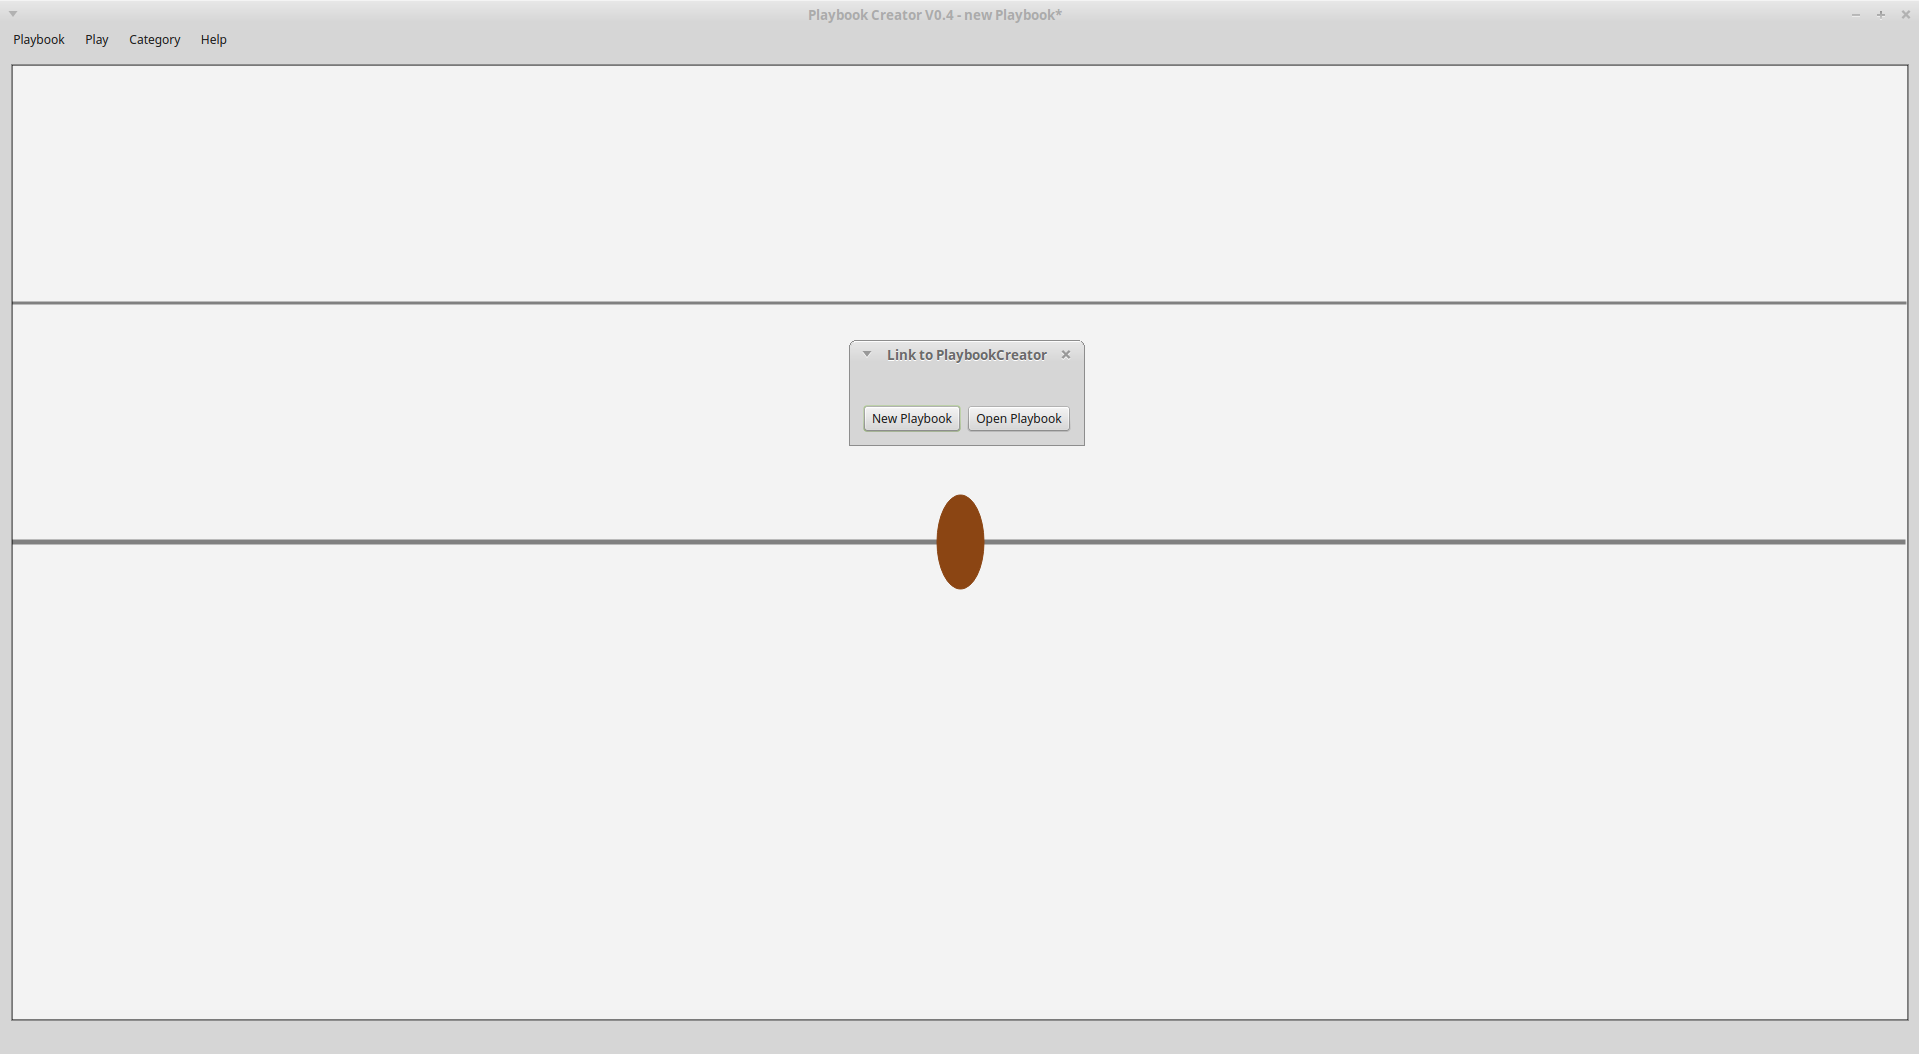
\includegraphics[scale=.2]{images/appStart.png}
			\caption{Application start}
			\label{fig:appStart}
		\end{figure}		
		If you created a playbook yet, you can click \textit{Open Playbook} and select your previously saved playbook file (*.pbc). If you want to create a new one click \textit{New Playbook} and enter the name of your playbook in the next dialog. \\
		
		In the next sections you will find detailed descriptions of the basic operations necessary to create a playbook. In section \ref{sec:guideline} there is a list of steps that are recommanded to create a playbook in an efficient way. You can also use it as a quick start guide if you want to skip the next sections. Because there is a little lack of usebility you should follow these steps (especially when you are new to Playbook Creator) to avoid repeating the same work everytime something failed due to early programming bugs.
		Sorry for that..but we are still in alpha developement stage ;-)
	\clearpage
	\section{Create a new play}
	\section{Apply a route to a receiver}
	\label{sec:routes}
		\subsection{Graphical}
		\subsection{Numerical}
	\section{Apply a motion to a receiver}
	\label{sec:motions}
	\section{Save Formations}
	\section{Export your playbook}
	\label{sec:pdfExport}
	\clearpage
	\section{Guideline for creating a new playbook}
	\label{sec:guideline}
		When creating a new playbook you should start with the following steps
		\begin{enumerate}
			\item Create your formations.
				\begin{enumerate}
					\item Click \textit{Play \pfeil New Play} and choose \textit{PBC\_Standardformation} (the only formation option you have)
					
					\item If you want to use colors to identify your players, assign the colors now by right-clicking on the player and then click \textit{Set Color}
					
					\item You can now change the position of the players either by drag\&drop or by right-clicking on the player and choosing \textit{Set Position}. The latter allows you to set the player's position exactly (measured in yards from the spot of the ball).
					
					\item Click on \textit{Play \pfeil Save Formation As} to add the current formation to your playbook. (Remember: if this is the first time that you add something like a formation, a route or a play to your playbook, Playbook Creator asks you to save it to disk.)
					
					\item Continue moving players and saving formations until you added all your desired formations to your playbook.
				\end{enumerate}
			\item Create your routes. You can also create your routes as you need them while creating plays, but it is recommended to do it prior to creating plays. You can create routes graphically or numerically by right-clicking on an arbitrary player, hovering over the \textit{Apply Route} menu item and selecting the right option from the sub menu. See section \ref{sec:routes} for further description. Repeat until you finished your route tree.
			
			\item Create your plays.
				\begin{enumerate}
					\item In the main menu click \textit{Play \pfeil New Play}. After typing name and code name of the play, choose one of the formations you created previously. Now you can bring the players in the ultimate position for the specific play you want to design. (Sometimes you want to change the alignment of a specific player or make some other little changes to the formation concerning the play. Then the play still remains associated with the chosen formation.)
					
					\item Apply motions to the receivers. See section \ref{sec:motions} for more information about how to create motions.
					
					\item Apply the routes you created in the previous step.
					
					\item When your done with designing your play, save it.
					
					\item Sometimes you want to design a play that looks similar to another one that you already designed. If you have that already designed play open, thats fine. Otherwise click \textit{Play \pfeil Open Play} in the main menu and open it. Now make your changes to it and save ot under a new name: click \mbox{\textit{Play \pfeil Save Play \textbf{As}}} and assign a new name and code name to it. You will see no changes in the displayed code name below your play (this is a bug), but your new play is saved under the new name. You can check that by clicking \textit{Play \pfeil Open Play}. You will see the new play and the old play which remains unchanged.
				\end{enumerate}
				
			\item Save your playbook. As you can read in previous sections of this document, you don't need to save your playbook explicitly. It is automatically saved when you add a play, route or formation to it. If you want to save your playbook despite automatic saving (e.g. to make a backup) you can click \mbox{\textit{Playbook \pfeil Save Playbook As}}.
			
			\item Export to PDF. Click \textit{Playbook \pfeil PDF Export} to open the export dialog. See section \ref{sec:pdfExport} for a detailed description of the export dialog. It is recommended to select some random plays (e.g. the first x plays) and export them to see if the export parameters you chose are correct. If feel certain about the parameters, open the export dialog again, select the plays you want and export them.
		\end{enumerate}
\end{document}